%%
%% Copyright 2007, 2008, 2009 Elsevier Ltd
%%
%% This file is part of the 'Elsarticle Bundle'.
%% ---------------------------------------------
%%
%% It may be distributed under the conditions of the LaTeX Project Public
%% License, either version 1.2 of this license or (at your option) any
%% later version.  The latest version of this license is in
%%    http://www.latex-project.org/lppl.txt
%% and version 1.2 or later is part of all distributions of LaTeX
%% version 1999/12/01 or later.
%%
%% The list of all files belonging to the 'Elsarticle Bundle' is
%% given in the file `manifest.txt'.
%%
%% Template article for Elsevier's document class `elsarticle'
%% with numbered style bibliographic references
%% SP 2008/03/01

\documentclass[preprint,12pt, a4paper]{elsarticle}

%% Use the option review to obtain double line spacing
%% \documentclass[authoryear,preprint,review,12pt]{elsarticle}

%% For including figures, graphicx.sty has been loaded in
%% elsarticle.cls. If you prefer to use the old commands
%% please give \usepackage{epsfig}

%% The amssymb package provides various useful mathematical symbols
\usepackage{amssymb}
\usepackage{hyperref}

\usepackage{graphicx}
\usepackage{caption}
\usepackage{subcaption}
\usepackage{listings}

%% The amsthm package provides extended theorem environments
%% \usepackage{amsthm}

%% The lineno packages adds line numbers. Start line numbering with
%% \begin{linenumbers}, end it with \end{linenumbers}. Or switch it on
%% for the whole article with \linenumbers.
%\usepackage{lineno}

\lstset{
  basicstyle=\ttfamily,
  frame=none,
  breaklines=true,
  numbers=left,
  xleftmargin=2.5em,
  framexleftmargin=0em,
  emphstyle=\textbf,
  float=t
  %  ,escapeinside={/*}{*/}
  ,moredelim=[is][\bfseries]{(*}{*)}
}
\lstdefinestyle{egx}{
  basicstyle=\ttfamily\scriptsize,
  emph={
    rule, transform, template, parameters, Map, Sequence, :
  },
  commentstyle=\sffamily\textit,
  comment=[l]{\#}
}
\lstdefinestyle{egl}{
  basicstyle=\ttfamily\scriptsize
}
\lstdefinestyle{model}{
  basicstyle=\ttfamily\scriptsize,
  emph={
    <, ?, xml, SocialNetwork, >, xmi, :, id, name, =, likes, dislikes, /,
    people, encoding, version, xmlns
  },
}
\lstdefinestyle{picto}{
  basicstyle=\ttfamily\scriptsize,
  emph={
    <, ?, /, :, >, =,
    nsuri, picto, format, icon, view, path, parameter, values,
    name, format, position, source, transformation, type
  },
}

\hyphenation{
  File-Watch-er Trans-form-er View-Con-tent-Cache Pic-to-Con-trol-ler
}


\journal{Science of Computer Programming}

% Science of Computer Programming
% Software Track Template for Short Paper
% Before you complete this template, a few important points to note:
% *  This template is for the short paper associated with an original software.
% If you are submitting an update to a software that has already been published,
% please use the software update template.
% *  The nature of a short paper associated with a software submission is very
% different to a traditional research article. To help you write yours,
% we have created this template. We will consider only software accompanied by
% short papers written using this template. However, it is acceptable
% to rename the section titles to something that is more specific to
% your software.
% •  In particular, remember that the goal of the paper is that it supports the submission of your software. It’s your software that will be evaluated, and the accompanying paper is only a part of the process.
% •  We strongly advise to make this short paper not longer than 6 pages.
% *  It is mandatory to publicly share the code and software referred to in your
% software article. You'll find information on our software sharing criteria in
% the Guide for Authors:
% https://www.elsevier.com/journals/science-of-computer-programming/0167-6423/guide-for-authors
% *  It's important to consult the Guide for Authors when preparing your
% submission; it highlights mandatory requirements and is packed with useful advice.
%
% Still got questions? Email our editorial team at scico.editors@gmail.com.
%
%Now you are ready to fill in the template below. As you complete each section,
% please carefully read the associated instructions. All sections are mandatory,
% unless marked optional.

\begin{document}

\begin{frontmatter}

%% Title, authors and addresses

%% use the tnoteref command within \title for footnotes;
%% use the tnotetext command for theassociated footnote;
%% use the fnref command within \author or \address for footnotes;
%% use the fntext command for theassociated footnote;
%% use the corref command within \author for corresponding author footnotes;
%% use the cortext command for theassociated footnote;
%% use the ead command for the email address,
%% and the form \ead[url] for the home page:
%% \title{Title\tnoteref{label1}}
%% \tnotetext[label1]{}
%% \author{Name\corref{cor1}\fnref{label2}}
%% \ead{email address}
%% \ead[url]{home page}
%% \fntext[label2]{}
%% \cortext[cor1]{}
%% \address{Address\fnref{label3}}
%% \fntext[label3]{}

\title{Exploring Complex Models with Picto Web}

%% use optional labels to link authors explicitly to addresses:
%% \author[label1,label2]{}
%% \address[label1]{}
%% \address[label2]{}

\author{Alfa Yohannis, Dimitris Kolovos, Antonio García-Domínguez,\\
  Carlos Javier Fernández Candel}

\address{University of York, United Kingdom}

\begin{abstract}
%% Text of abstract
Exploring and visualising a complex model in a single view can be challenging as it can require a considerable amount of computational resources and make the model difficult to comprehend due to information overload.
Picto Web is a tool designed for complex model exploration. Using the Epsilon Generation Language for model-to-text transformation, it can transform domain-specific models into multiple transient web-based views in different formats, such as HTML, Graphviz, and PlantUML. 
Picto Web uses lazy and incremental model-to-text transformation to (re)generate views efficiently. 
Moreover, it supports push notifications to clients when views are updated and is packaged as a Docker container for ease of use.
\end{abstract}

\begin{keyword}
%% keywords here, in the form: keyword \sep keyword - maximum of six
%keyword 1 \sep keyword 2 \sep keyword 3
complex models \sep model exploration \sep picto \sep web \sep visualisation
\end{keyword}

\end{frontmatter}

%\linenumbers

\section*{Metadata}
\label{}

This ancillary data table is required for the sub-version of the codebase.
Please replace the text in the right column with the correct information
about your current code and leave the left column untouched.

\begin{table}[!h]
\begin{tabular}{|l|p{6.5cm}|p{6.5cm}|}
\hline
\textbf{Nr.} & \textbf{Code metadata description} & \textbf{Please fill in this column} \\
\hline
C1 & Current code version & 0.1.02-SCP\\
\hline
C2 & Permanent link to code/repository used for this code version & $https://github.com/epsilonlabs/picto\-web$ \\
\hline
C3  & Permanent link to Reproducible Capsule & \\
\hline
C4 & Legal Code License   & Eclipse Public License (EPL-2.0) \\
\hline
C5 & Code versioning system used & git \\
\hline
C6 & Software code languages, tools, and services used & Java, Javascript, HTML, CSS, Graphviz \\
\hline
C7 & Compilation requirements, operating environments and dependencies & Java 11, Maven \\
\hline
C8 & If available, link to developer documentation/manual & For example: $https://github.com/epsilonlabs/picto\-web$ \\
\hline
C9 & Support email for questions & Online forum $https://www.eclipse.org/forums/index.php/f/22/$\\
\hline
\end{tabular}
\caption{Code metadata}
\label{}
\end{table}

\section{Motivation and significance}
%In this section, we want you to introduce the scientific background and the
%motivation for developing the software.
%
%\begin{itemize}
%  \item Explain why the software is important and describe the exact
%      (scientific) problem(s) it solves.
%
%  \item Indicate in what way the software has contributed (or will contribute
%      in the future) to the process of scientific discovery; if available,
%      please cite a research paper using the software.
%
%  \item Provide a description of the experimental setting. (How does the user
%      use the software?)
%
%  \item Introduce related work in literature (cite or list algorithms used,
%      other software, and so on).
%\end{itemize}

A model is commonly considered complex when it has a large number of heterogeneous elements which are involved in non-trivial relationships \cite{boccara2010complex,klosterman2012complex}. One way to understand and communicate such models is through visualisation. However, displaying all elements and their relationships in a single graphical representation is often undesirable since it can overload users with information and make visualisations challenging to comprehend. In terms of computation, this approach is also inefficient for large models since a potentially very large and complex diagram (or similar visual representation) has to be rendered in one go. 
Moreover, in a multi-user environment, the visualisation also has to deal with multiple, repeated requests, whether a user is refreshing a view or different users requesting the same view over the network.
Thus, novel mechanisms are necessary to allow engineers and other stakeholders to develop and perform contextual exploration of complex models from different viewpoints and at varying levels of detail. The visualisation also should be able to handle repeated requests from multiple users and return the requested views promptly.

There has been some work related to complex model exploration. For example, Sprotty~\cite{sprotty2022git} is an open-source diagramming framework that uses web technologies to render graphical views. 
Besides being used on the client-side for fast, scalable SVG rendering with ELK layout, it also provides a headless component that can be used for integration with the Xtext framework, extending Language Server Protocol, and computing diagram layout on the server side. Sprotty only supports node-edge diagrams and does not support rendering views conforming to different technologies, such as tables in HTML, PlantUML and Graphviz diagrams. Moreover, Sprotty does not support semantic editing on diagrams. As an alternative, the Graphical Language Server Platform (GLSP)~\cite{eclipse2022glsp} allows complete control and access over the Sprotty diagrams and can be considered if diagram editing via web browsers is required.

The KIELER Lightweight Diagram (KLD) framework~\cite{schneider2013just} uses Xtend, Piccolo2D and EMF to allow on-demand model visualisation, and also the KIELER Infrastructure for Meta Layout (KIML) for defining diagram layouts. KLD uses three EMF-based models (KLayoutData, KRendering, and KGraph) for users to describe a diagram. KLD is also extensible via Java/Xtend interfaces, which should be implemented to transform and map a semantic model to KGraph and KRendering models. Similar to Sprotty, KLD only supports rendering views in node-edge diagrams. As a comparison, Picto and Picto Web support rendering views in multiple formats, such as table/form views in HTML, PlatUML and Graphviz diagrams, and views generated using JavaScript graphical libraries, e.g., Three.js.

\begin{figure}
  \centering
  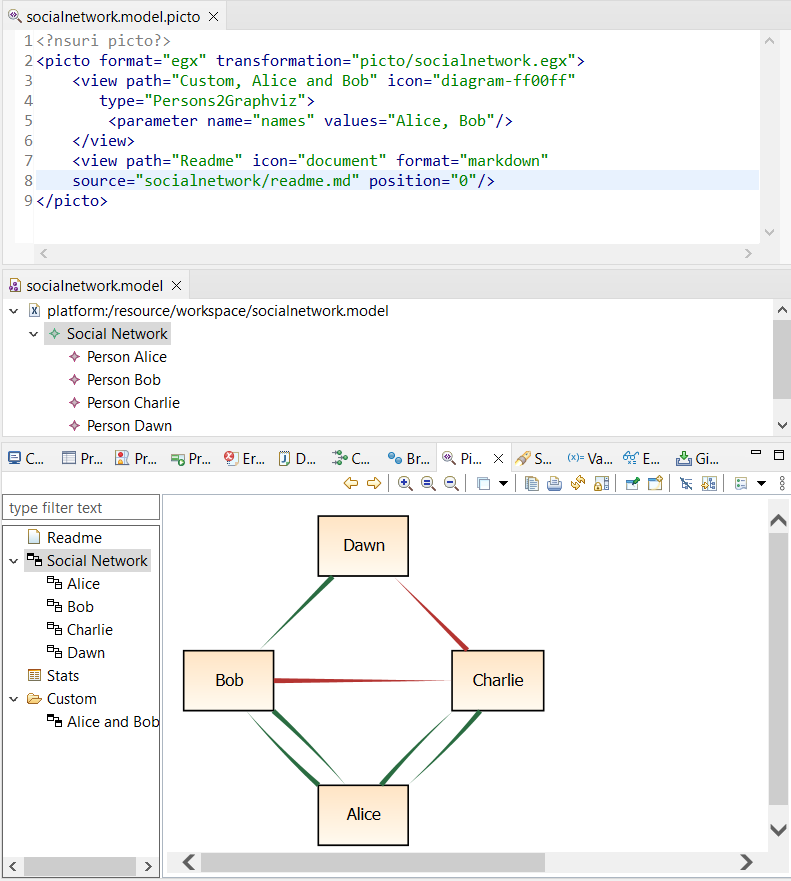
\includegraphics[width=\linewidth]{images/picto-eclipse.png}
  \caption{Picto plugin for Eclipse environment.
  }
  \label{fig:picto-eclipse}
\end{figure}

Picto \cite{dimitris2020picto} is another visualisation tool, which is an Eclipse plugin, that uses lazy model-to-text transformation to generate transient graphical views from heterogeneous models. Figure \ref{fig:picto-eclipse} shows a screenshot of Picto within Eclipse. 

Picto’s user interface has two main components. On its left-hand side is a tree widget that displays the titles and icons of the views (Social Network, Alice, Bob, Charlie and Dawn) that users can select from. Once a view is selected, its content is generated and rendered in an embedded web browser -- through a series of transformations -- on the right-hand side of Picto. In Figure \ref{fig:picto-eclipse}, the selected view visualises the entire model in the form of a Graphviz-based node-edge diagram. Beyond Graphviz, Picto also supports PlantUML and SVG/HTML as visualisation formats, and also features an extensible architecture that enables adopters to extend it with additional diagram-as-code formats.  

A challenge with Picto is that it is implemented as a plugin of the Eclipse IDE, which means that for engineers to use it, they need to install Java, Eclipse and Picto and check out the models they wish to explore (as well as the respective visualisation transformations) locally. While this is not an issue for software developers who are already familiar with Eclipse, it can represent a significant barrier for other engineers and stakeholders. 

In this paper, we present Picto Web\footnote{\url{https://github.com/epsilonlabs/picto-web}}, a web-based version of the Picto\footnote{\url{https://www.eclipse.org/epsilon/doc/picto}} \cite{dimitris2020picto} model visualisation tool which was originally implemented as an extension of the Eclipse IDE. Unlike Picto, Picto Web does not require local software installation, which makes it more suitable for a broader audience of developers and stakeholders who would benefit from access to dynamically-generated graphical views of complex software and system models.

\section{Software description}
%Describe the software. Provide enough detail to help the reader understand
%its impact.
Picto Web maintains the core features of the Eclipse-based version of Picto, such as supporting the lazy generation of views, drilling-up/down tree views, multi-views, and multi-formats, but it is implemented as a multi-tenant client-server web application that can be accessed through a standard web browser to perform interactive complex model exploration. 
Picto Web monitors model files and visualisation model-to-text templates for changes and immediately propagates any updates to generated views to the viewers' web browsers, delivering a live user experience.

\subsection{Software architecture}
%Give a short overview of the overall software architecture; provide a
%pictorial overview where possible; for example, an image showing the
%components. If necessary, provide implementation details.
The architecture of Picto Web is displayed in Figure \ref{fig:architecture} and consists of two parts: a server-side part that lazily runs visualisation transformations against models, and a browser-based client that displays the visualisation results. 

\begin{figure}[h]
  \centering
  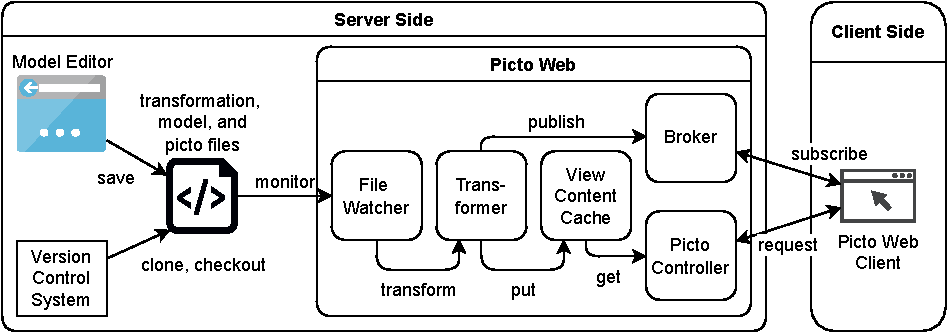
\includegraphics[width=\linewidth]{images/architecture.pdf}
  \caption{The architecture of Picto Web.}
  \label{fig:architecture}
\end{figure}

The server-side part of Picto Web consists of the \texttt{File\-Watch\-er}, \texttt{Trans\-form\-er}, \texttt{View\-Con\-tent\-Cache}, \texttt{Picto\-Control\-ler}, and \texttt{Broker} components shown on the left hand side of the figure. The \texttt{File\-Watcher} component is responsible for monitoring a directory that contains the models that Picto Web needs to visualise (see Section \ref{sec:transformation}). When any of the files is modified (added, deleted, or updated), \texttt{FileWatcher} detects the change and notifies the \texttt{Transformer} component, which then generates, refreshes, or invalidates the contents of the respective views\footnote{The mechanisms used to implement incremental view invalidation and re-generation upon changes in models and templates are based on the work in \cite{ogunyomi2019}, but a detailed description is beyond the scope of this paper.}.

After that, Picto Web puts the generated views into a cache (\texttt{View\-Content\-Cache}) that maps the paths of the views in the tree view to their actual contents. The cache is used to avoid wastefully re-generating views which cannot have been impacted since the last time a client requested them. Therefore, Picto Web can respond promptly to multiple, repeated requests for the same views. 

Every time a client requests the content of a specific view, \texttt{Picto\-Control\-ler} receives and handles the request by retrieving the view content from \texttt{View\-Content\-Cache} using the view's path sent in the request as the key for the map. The retrieved content is then returned to the client to display.

\texttt{Broker} is a component responsible for pushing updates to Picto Web clients. Every time a Picto Web client starts visualising a model, the client subscribes to the \texttt{Broker} so that it can receive further updates from the Picto Web server-side component if any of the model files are subsequently modified. After transformation, the \texttt{Transformer} publishes new content views to the \texttt{Broker}.

We have packaged the Picto Web server in the form of a Docker image\footnote{\url{https://hub.docker.com/r/alfayohannisyorkacuk/picto-web}} so that users can easily deploy and test it using the following command. 

\begin{verbatim}
  docker run --rm -it -v $PWD:/workspace -p 8080:8080 picto-web
\end{verbatim}

The Picto Web server can then be accessed via \texttt{http://localhost:8080} on a web browser. 
The \texttt{-v \$PWD:/workspace} option is used to allow the Docker image to access the transformation and model files in the current directory from its internal \texttt{/workspace} directory. 
This way, the internal \texttt{FileWatcher} in the Picto Web Docker image can monitor the file system for any relevant changes that should trigger view generation or invalidation.

\subsection{Software functionalities}
%Present the major functionalities of the software.

In this example, we wish to visualise models conforming to a contrived social network metamodel from \cite{dimitris2020picto}. In particular, we use a sample model containing four people (Alice, Bob,  Charlie and Dawn) and like/dislike relationships between them. From such social network models we wish to produce one node-edge view for the entire social network, and one view for each member of the network that omits anyone they neither like nor dislike.

A social network model is a graph that contains a number of people as its nodes linked with \emph{like} and \emph{dislike} relationships. In a view, as shown in Figure \ref{fig:ui_social_network}, a person is depicted as a rectangle while the \emph{like} and \emph{dislike} relationships are presented as green and red edges respectively. This node-edge view is the visualisation of the social network model defined in Listing \ref{lst:model}.

\begin{figure*}[h]
  \centering
  \hfill
  \begin{subfigure}{0.49\textwidth}
    \frame{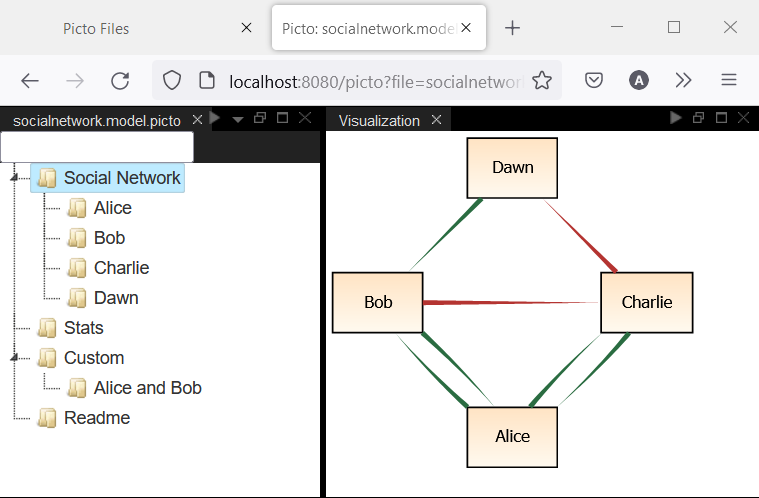
\includegraphics[width=\textwidth]{images/gui-social-network.png}}
    \caption{the overall social network}
    \label{fig:ui_social_network}
  \end{subfigure}
  \hfill
  \begin{subfigure}{0.49\textwidth}
    \frame{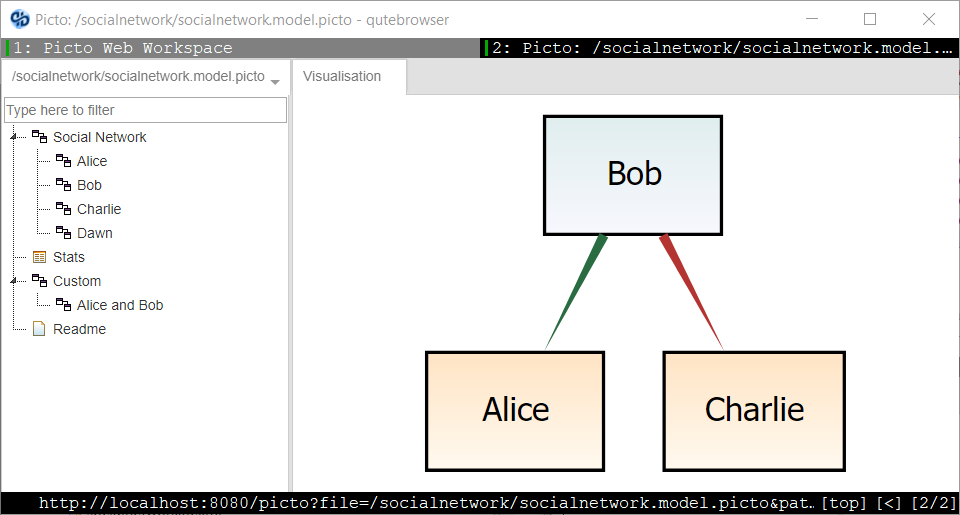
\includegraphics[width=\textwidth]{images/gui-bob.png}}
    \caption{Bob's social network}
    \label{fig:ui_bob}
  \end{subfigure}
  \hfill
  \begin{subfigure}{0.49\textwidth}
    \frame{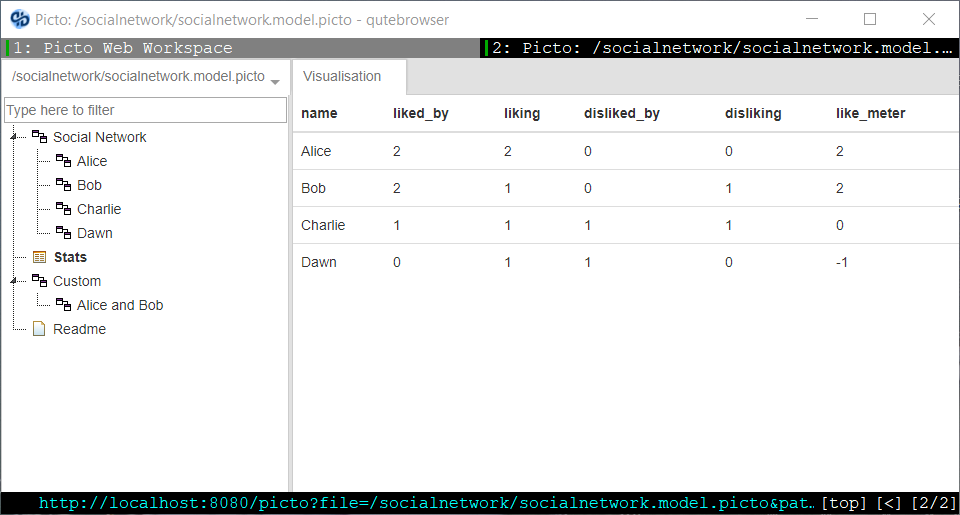
\includegraphics[width=\textwidth]{images/gui-tabular.png}}
    \caption{an HTML table summarising the social network}
    \label{fig:ui_tabular}
  \end{subfigure}
  \hfill
  \begin{subfigure}{0.49\textwidth}
    \frame{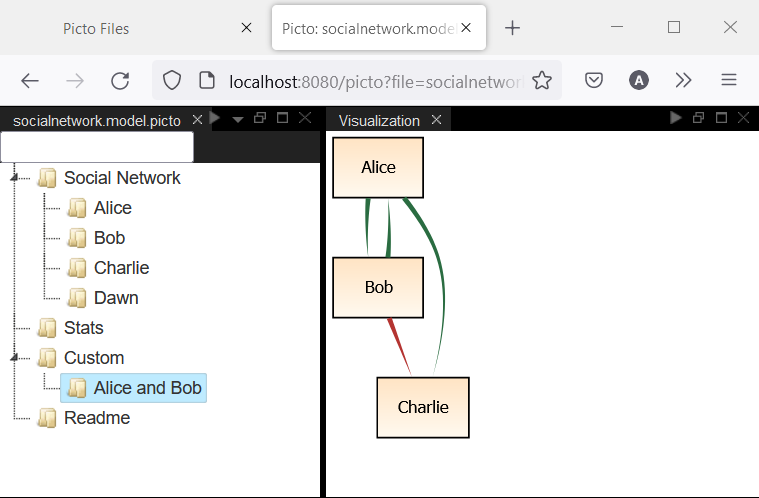
\includegraphics[width=\textwidth]{images/gui-custom.png}}
    \caption{custom Alice and Bob's social network}
    \label{fig:ui_custom}
  \end{subfigure}
  \hfill
  \caption{Picto Web client displays different views.}
  \label{fig:ui}
\end{figure*}

Figure \ref{fig:ui} shows the user interface of Picto Web, which has two main areas. The left side is a tree view which lists the views produced from the underpinning model(s) in a hierarchical way, and the right side is a panel that displays the content of the active, selected view. In our example, when a user selects the \emph{Social Network} view on the left hand side, Picto Web displays the overall social network of Alice, Bob, Charlie, and Dawn (Figure \ref{fig:ui_social_network}). 

Viewers can also drill down to display the local social network of each person through the tree view on the left. For example, Figure \ref{fig:ui_bob} displays Bob's social network. Besides being able to display view contents in SVG/HTML as in Figures \ref{fig:ui_social_network} and \ref{fig:ui_bob}, Picto Web is also able to render model views in other formats. For example, Figure \ref{fig:ui_tabular} displays a summary of the social network in the form of a HTML table. 

In addition to procedurally-generated views (e.g. one view for each person in the network), developers can also define custom views, as shown in Figure \ref{fig:ui_custom}. The figure is customised only to display the social network of Alice and Bob. 

%\subsection{Sample code snippets analysis or use cases of the software (optional)}
\subsection{Transformation}
\label{sec:transformation}

Picto requires at least three types of files: model files (any model representation format supported by Epsilon\footnote{\url{https://eclipse.org/epsilon/doc/emc}} is also supported by Picto Web), visualisation transformation files in Epsilon's EGL template-based language (*.egl, *.egx), and Picto files (*.picto) which bind models to visualisation transformations and specify custom views (EGL, EGX, and Picto files are explained briefly later in this section). Listing \ref{lst:model} shows the XMI-based representation of the social network model of our running example. 

The visualisation transformation consists of EGL (Epsilon Generation Language) templates ~\cite{rose2008egl} that produce individual views, and an EGX (EGL Co-Ordination Language)\footnote{\url{https://www.eclipse.org/epsilon/doc/egx}} program that specifies how the templates should be executed against different elements in the model(s). Listing \ref{lst:egx} shows an excerpt of the EGX transformation coordination program of this example. Rule \texttt{Network2Graphviz} runs the \texttt{socialnetwork2} \texttt{graphviz.egl} template of Listing \ref{lst:egl} for every \texttt{SocialNetwork} element in the source model and produces a Graphviz-based view for it. The EGL template of Listing \ref{lst:egl} defines the logic for generating the content of the view. An actual generated view in Graphviz is shown in Listing \ref{lst:output}. 

Picto files bind the transformation coordination and model files to generate the contents of the target views. In Listing \ref{lst:picto}, Picto Web uses the \texttt{socialnetwork.egx} transformation coordination file that contains the rule in Listing \ref{lst:egx} to transform the social network model in Listing \ref{lst:model} into the social network and individual person views shown in Figure \ref{fig:ui}. It also includes two additional views: (1) a custom view that includes only Alice and Bob's social network (Figure \ref{fig:ui_custom}) and (2) a view that displays a Markdown readme file.
\begin{lstlisting}[firstnumber=1,style=model,caption={A social network model as the input file for the lazy transformation. The format of the ids is simplified.},label=lst:model,float]
<?xml version="1.0" encoding="ASCII"?>
<SocialNetwork xmlns="socialnetwork" xmi:id="sn">
  <people xmi:id="a" name="Alice" likes="b c"/>
  <people xmi:id="b" name="Bob" likes="a" dislikes="c"/>
  <people xmi:id="c" name="Charlie" likes="a" dislikes="d"/>
  <people xmi:id="d" name="Dawn" likes="b"/>
</SocialNetwork>
\end{lstlisting}
\begin{lstlisting}[firstnumber=1,style=egx,caption={The Network2Graphviz EGX rule},label=lst:egx,float]
rule Network2Graphviz 
transform n : socialnetwork::SocialNetwork {
  template : "socialnetwork2graphviz.egl"
  parameters : Map{
    "path" = Sequence{"Social Network"},
    "format" = "graphviz-circo",
    "people" = n.people
  }
}
\end{lstlisting}
\begin{lstlisting}[firstnumber=1,style=egx,caption={An EGL template that generates a Graphviz representation of a social network.},label=lst:egl,float]
digraph G {
  node[shape=rectangle, fontname=Tahoma, fontsize=10, style="filled", gradientangle="270", fillcolor="bisque:floralwhite"]
  edge[penwidth=3, style=tapered, arrowhead=none]
  (*[%for (p in people){%]*)
    (*[%=p.name%]*)
    (*[%for (l in p.likes){%]*)
      (*[%=p.name%] -> [%=l.name%]*) [color=green]
      (*[%}%]*)
    (*[%for (l in p.dislikes){%]*)
      (*[%=p.name%] -> [%=l.name%]*) [color=red]
    (*[%}%]*)
  (*[%}%]*)
}
\end{lstlisting}
\begin{lstlisting}[firstnumber=1,style=egx,caption={A view generated by the EGL template in Listing \ref{lst:egl}.},label=lst:output,float]
digraph G {
  node[shape=rectangle, fontname=Tahoma, fontsize=10, style="filled", gradientangle="270", fillcolor="bisque:floralwhite"]
  ...
  Alice
  Alice -> Bob [color=green]
  ...
  Dawn
  Dawn -> Bob [color=green] 
}
\end{lstlisting}
\begin{lstlisting}[firstnumber=1,style=picto,caption={The Picto file that binds the model and the visualisation transformation.},label=lst:picto,float]
<?nsuri picto?>
<picto format="egx" transformation="picto/socialnetwork.egx">
  <view path="Custom, Alice and Bob" icon="diagram-ff00ff" type="Persons2Graphviz">
    <parameter name="names" values="Alice, Bob"/>
  </view>        
  <view path="Readme" icon="document" format="markdown" source="socialnetwork/readme.md" position="0"/>
</picto>
\end{lstlisting}

\section{Illustrative examples}
%Provide at least one illustrative example to demonstrate the major functions
%of your software/code. If you wish to include a video to supplement your
%Original Software Publication, please ensure the file is included as
%supplementary material or provide a link to your video in this
%section.
%This section can also refer to/summarize already published examples and case studies.
\begin{figure}[h]
  \centering
  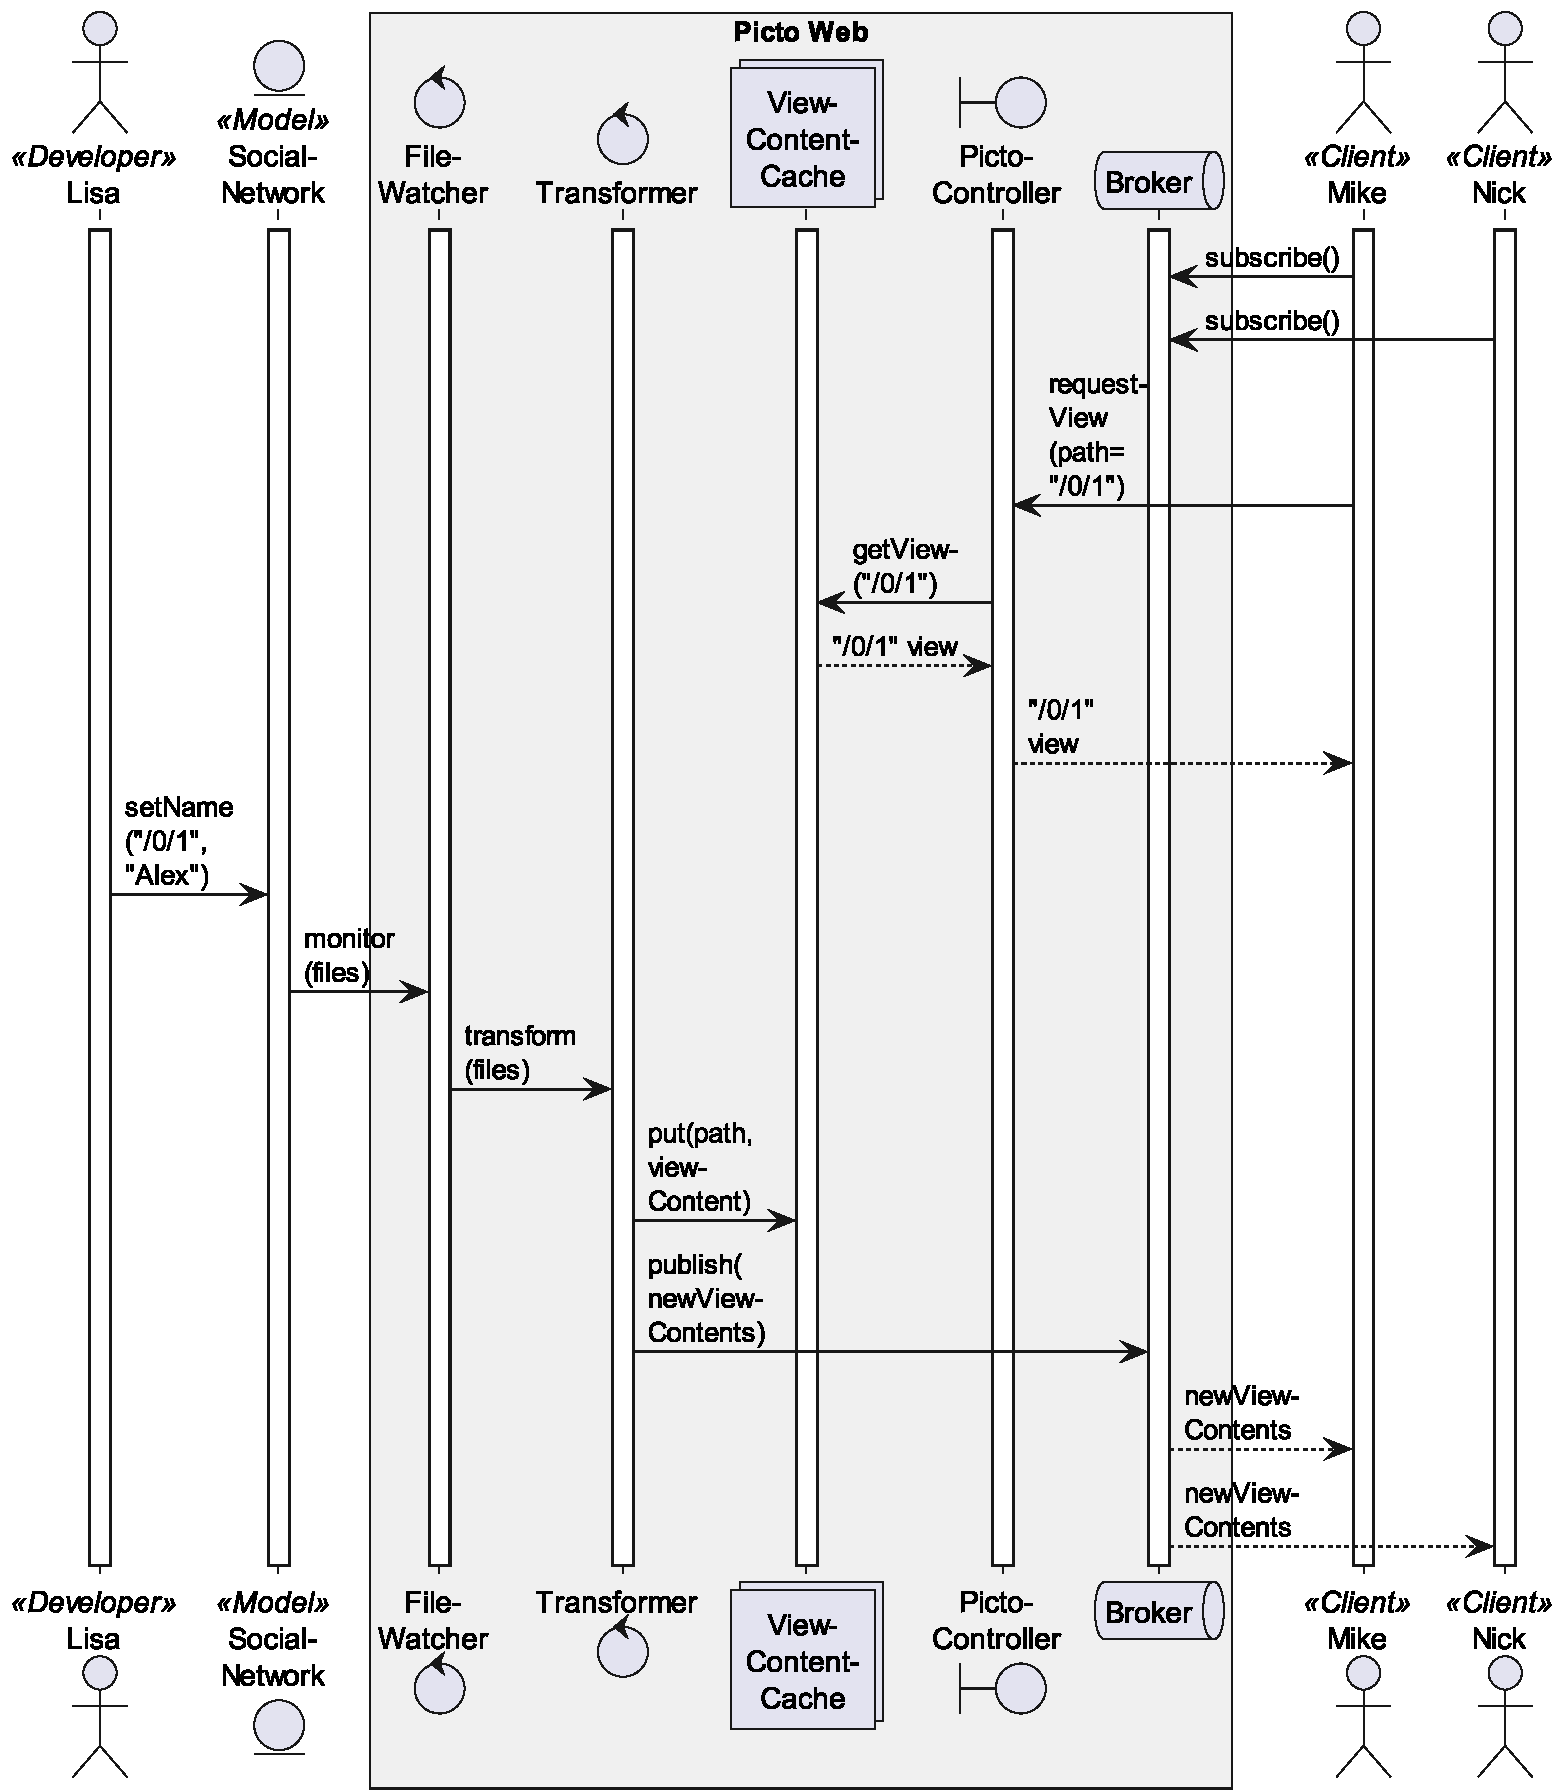
\includegraphics[width=1\linewidth]{images/sequence}
  \caption{Requests and Updates of Picto Web's view contents.}
  \label{fig:sequence}
\end{figure}

This section demonstrates Picto Web's internal control flow, visualised in the sequence diagram of Figure \ref{fig:sequence}. Suppose that the \texttt{ViewContentCache} has been populated with view contents through an initial transformation executed when a developer (Lisa) created the social network model -- the process is not displayed in the diagram. Stakeholders Mike and Nick wish to explore Lisa's model and start running Picto Web clients. The clients subscribe to the broker provided by the Picto Web server application so that they can receive further updates on the model. 

Mike is interested in knowing more about Alice's social network. Therefore, he sends a view request to Picto Web with a parameter containing Alice's view path, ``/0/1''\footnote{Simplified format}. Since the view content of the path is already available in the \texttt{View\-Content\-Cache} from the initial transformation, \texttt{Picto\-Controller} (the component that handles the request) retrieves Alice's view content from the cache and sends it back to Mike's client to be displayed.

At some point, Lisa decides to rename ``Alice'' to ``Alex'' and save the change to the model file. \texttt{File\-Watcher} detects that the file has been modified and notifies the \texttt{Transformer} to generate new view contents from the modified file and update the \texttt{View\-Content\-Cache}. The \texttt{Transformer} also publishes the new content views to the \texttt{Broker} so that the subscribers, Mike and Nick, also receive the new content views and perform live updates on the view contents they currently display.

\section{Impact}
Picto Web is expected to bring impact complex model exploration in model-driven engineering. Some improvements that it delivers over existing tools\cite{sprotty2022git,schneider2013just,dimitris2020picto} are: 
\begin{enumerate}
\item It allows users to develop and perform contextual exploration of complex models at varying levels of detail and from different viewpoints.
\item It supports the visualisation of various models in different representation formats (e.g., HTML, Graphviz, SVG, PlantUML, etc.).
\item It is a multi-user environment and immediately propagates any updates on models to viewers, delivering a live user experience. 
\end{enumerate}

The capabilities are promising to bring changes to daily practices in the industry as viewers are concerned with different aspects or parts of models, 
and they can view the current state of the models in a live manner. 
For example, in visualising the current state of a particular software part, 
a user prefers to view a model in state charts, 
while another viewer favours sequence diagrams. 
Both can immediately receive the model's current state when it is modified.
Another research area worth exploring is how to extend the visualisation to perform model differencing to tell viewers which parts of the models have recently changed.

%This is the main section of the article and reviewers will weigh it
%appropriately. Please indicate:
%
%\begin{itemize}
%  \item Any new research questions that can be pursued as a result of your
%      software.
%
%  \item In what way, and to what extent, your software improves the pursuit
%      of existing research questions.
%
%  \item Any ways in which your software has changed the daily practice of
%      its users.
%
%  \item If applicable, how widespread the use of the software is within and
%      outside the intended user group (downloads, number of users if your
%      software is a service, citable publications, and so on).
%
%  \item If applicable, how the software is being used in commercial
%      settings or how it has led to the creation of spin-off companies.
%      Please note that points 1 and 2 are best demonstrated by references
%      to citable publications. \end{itemize}

\section{Conclusions}
In this paper, we presented Picto Web, a web-based version of the Picto model visualisation tool which was originally implemented as a plug-in of the Eclipse IDE. Unlike Picto, Picto Web does not require local software installation, which makes it more suitable for a broader audience of developers and stakeholders who would benefit from access to dynamically-generated graphical views of complex software and system models. 

\section{Future Plans}
%Your future plans to expand the software.
Going forward, we plan to further improve the performance of visualisation transformations in Picto Web by establishing an element/property access trace of the visualisation transformations, to enable more fine-grained regeneration and invalidation of generated views.

\section*{Acknowledgements}
\label{}
%You can use this section to acknowledge colleagues who do not qualify as a
%co-authors but helped you in some way. Optionally thank people and institutes
%you need to acknowledge.
The work in this paper has been funded through the HICLASS InnovateUK project (contract no. 113213).

\section*{References}

%If the software repository you used supplied a DOI or another Persistent
%IDentifier (PID), please add a reference for your software here. For more
%guidance on software citation, please see our guide for authors or this
%article on the essentials of software citation by FORCE 11, of which Elsevier
%is a member.

%% References:
%% If you have bibdatabase file and want bibtex to generate the
%% bibitems, please use
%%
  \bibliographystyle{elsarticle-num}
  \bibliography{bibliography}

%% else use the following coding to input the bibitems directly in the
%% TeX file.

%\begin{thebibliography}{00}
%
%%% \bibitem{label}
%%% Text of bibliographic item
%
%\bibitem{}
%
%\end{thebibliography}

\end{document}
\endinput
%%
%% End of file `SoftwareX_article_template.tex'.
